% Origen: sección "Apéndice" de Secciones/PI - Implementacion MCA.md
% Archivo apend7 por orden de creación; en template.tex va después de apend3.
% Lo que en la nota está entre %% (datapath del trapecio, funcionamiento interno
% del conformado trapezoidal, criterio de separación, elección de parámetros)
% no se transcribe.
\chapter{Detalles del MCA}
\label{C:ap-mca}

% Figuras de este apéndice + las compartidas.
\graphicspath{{figs/apendices/}{figs/comunes/}}

\section{Detección de solape en HW}
\label{S:ap-mca-solape}

Las marcas de solape no miran la señal sino los disparos del MT: un pulso que el
MT no disparó, por ejemplo porque llegó durante su re-armado, no deja marca. Se
calculan en dos lugares. Lo que se sabe al abrir lo decide \codigo{mca\_window},
una sola vez para todas las ranuras, y se registra junto con la muestra del
disparo; lo que pasa durante la ventana lo anota cada ranura. Las distancias se
cuentan en muestras válidas y saturan en \codigo{0xFFFF}.
\begin{itemize}
  \item \textbf{Distancia al disparo anterior, \codigo{dt\_prev}.}
    \codigo{mca\_window} tiene un contador común que suma uno por muestra válida
    y vuelve a cero con cada disparo, haya abierto ranura o no, incluso bajo
    veto. En la muestra de un disparo, su valor más uno es la distancia al
    anterior, y la ranura que abre la copia. Antes del primer disparo vale
    \codigo{0xFFFF}.
  \item \textbf{Ranuras abiertas al abrir, \codigo{otras}.} El asignador cuenta
    las ranuras abiertas o reservadas en el ciclo en que decide abrir. Las
    cerradas no cuentan, porque su ventana ya terminó y no se superpone con la
    nueva. Satura en 4 bits.
  \item \textbf{Disparo adentro, \codigo{adentro} y \codigo{dt\_next}.} Mientras
    la ranura mide, cada disparo que llega con la ventana abierta marca
    \codigo{adentro}, y el primero copia el largo de la ventana en ese momento,
    \codigo{len}, en \codigo{dt\_next}, que arranca en \codigo{0xFFFF}. No
    cuentan el disparo que abrió la ranura, que llega cuando todavía figura
    libre, ni uno en la muestra de cierre, que ya no es de la ventana.
  \item \textbf{Disparo perdido, \codigo{perdido}.} Si un disparo no encuentra
    ranura libre (y no hay veto), el asignador lo marca, y lo anotan todas las
    ranuras que en ese momento están abiertas: el pulso que se perdió está
    montado sobre ellas, y su carga entra en lo que miden sin que quede otro
    registro de él.
\end{itemize}

Al cerrar, una ranura queda \textbf{superpuesta} si \codigo{otras} $\neq 0$ o si
llegó un disparo adentro. Esas ventanas se cuentan en \codigo{cnt\_pileup}, pero
se publican igual: la ranura no corrige nada, deja escrito en el resultado que
midió sobre otro pulso. En el bus, \codigo{F\_DTPREV} y \codigo{F\_DTNEXT}
llevan las dos distancias, y \codigo{F\_SOLAPE} las tres marcas, en el campo de
bits \{\codigo{perdido}[5], \codigo{adentro}[4], \codigo{otras}[3:0]\}. Las usan
la elección de la forma del banco, que compara las distancias contra los
umbrales de cada forma, y el discriminador o el software, que pueden descartar
los eventos marcados. \codigo{dt\_next} sólo ve disparos dentro de la ventana,
así que un vecino que llega después del cierre no aparece; por eso los umbrales
$\text{después}_f$ del banco no pueden superar a \codigo{gate\_long}, y el bit
31 de \codigo{cfg\_n\_formas} avisa si alguno lo hace.

\section{Modelos de tiempo muerto}
\label{S:ap-mca-modelos}

Los modelos de tiempo muerto (Sec.~\ref{S:mca-modelos-tiempo-muerto}) son una
predicción del tiempo muerto real, que es el que mide el teselado: a partir de
la tasa de disparos y del largo de la ventana dicen cuánto tiempo muerto
esperar. Sirven para dimensionar el módulo, por ejemplo cuántas ranuras hacen
falta para una tasa dada, y para contrastar la medición: si el tiempo muerto
medido se aparta del predicho, el modelo no describe al sistema. Para decidir
qué modelo aplica están la ocupación de las ranuras y los tres contadores de los
períodos muertos. No son un histograma de largos sino su cantidad, su máximo y
su suma, porque los períodos son los mismos ciclos que suman a
$\mathtt{t\_win} + \mathtt{t\_div}$, y de ahí sale el largo medio sin
correcciones:
\begin{equation}
  E[L] = \frac{\mathtt{t\_win} + \mathtt{t\_div}}{\mathtt{cnt\_dead\_periods}}
  \label{e:ap-mca-largo-medio}
\end{equation}
\begin{itemize}
  \item \textbf{Con una ranura} el MCA es no paralizable: un disparo que llega
    con la ranura ocupada se pierde sin extender nada. Sin decimación, cada
    período dura exactamente $\tau = \mathtt{gate\_long} + 1 + 18$ ciclos (la
    ventana, la muestra de cierre y la publicación), así que
    $\mathtt{max\_dead\_len} = E[L] = \tau$, y la igualdad verifica el modelo en
    cada adquisición.
  \item \textbf{Con $N$ ranuras} el MCA es un sistema de pérdida M/D/N/N: $N$
    servidores con servicio de largo $\tau$ y sin cola de espera. La fracción
    del tiempo con $j$ ranuras ocupadas, que mide directamente
    \codigo{t\_ocup[j]} (Sec.~\ref{S:ap-mca-ocupacion}), sigue la distribución
    de Erlang~\citecap{Kleinrock1975}{3}, y la pérdida es la fracción con las
    $N$ ocupadas.
    \begin{equation}
      p_j = \frac{\rho^j/j!}{\sum_{i=0}^{N}\rho^i/i!}, \qquad P_{MCA} = p_N,
      \qquad \rho = \lambda\tau
      \label{e:ap-mca-erlang}
    \end{equation}
    A tasa baja, $p_N \simeq \rho^N/N!$, contra $\simeq \rho$ con una ranura.
    Ahora un período arranca cuando se ocupa la última ranura libre y termina
    cuando se libera alguna, así que dura menos que una ventana y su largo es
    variable. El modelo no incluye al publicador: si varias ranuras cierran
    juntas, alguna espera y su servicio se alarga.
\end{itemize}

El disparo tiene su propio modelo, que depende de la fuente: la del MT se
presenta en la Sec.~\ref{S:mt-relanzamiento}.

\section{Contadores de ocupación de las ranuras}
\label{S:ap-mca-ocupacion}

Además de los casilleros del teselado, el módulo cuenta la ocupación de las
ranuras con dos relojes más, que no forman parte del teselado:
\begin{itemize}
  \item \codigo{t\_ocup[j]} cuenta los ciclos con exactamente $j$ ranuras
    ocupadas, fuera del veto. Es un segundo teselado, del tiempo no vetado según
    la ocupación, $\sum_j \mathtt{t\_ocup}[j] = T_{real} - T_{veto}$, y es el que
    mide la distribución de Erlang del modelo de $N$ ranuras
    (Sec.~\ref{S:ap-mca-modelos}). Con las $N$ ranuras habilitadas ocupadas no
    hay ninguna libre, así que $\mathtt{t\_ocup}[N] = \mathtt{t\_win} +
    \mathtt{t\_div}$.
  \item \codigo{deadtime} cuenta los ciclos con alguna ranura ocupada, fuera del
    veto. No es el tiempo muerto del módulo: con una ranura coincide con
    $\mathtt{t\_win} + \mathtt{t\_div}$, pero con varias el módulo puede abrir
    mientras otras ranuras miden. El nombre se conservó de cuando el módulo
    tenía una sola ranura.
\end{itemize}

\section{Primera versión del módulo (MCA1)}
\label{S:ap-mca-mca1}

La primera versión del módulo, a la que llamamos MCA1, medía un pulso a la vez y
no tenía banco de trapecios. Se presenta en la Fig.~\ref{f:ap-mca-mca1}, en el
mismo estilo que la Fig.~\ref{f:implmca-panorama} para poder compararlas. Las
diferencias con la versión actual son:
\begin{itemize}
  \item \textbf{Una sola ventana.} Mientras medía un pulso no podía abrir otra,
    así que un segundo pulso dentro de la ventana se perdía. Las ranuras
    multiplican esa ventana.
  \item \textbf{Quién abre.} Además del disparo externo, un Schmitt propio sobre
    $x$, con umbral e histéresis. Se sacó porque no puede ver un pulso montado
    sobre la cola de otro: la señal nunca baja del umbral entre los dos, y ver
    esos pulsos es para lo que están las ranuras. En las primeras versiones el
    Schmitt era el único, y la publicación, bloqueante; el disparo externo y la
    cola entraron después.
  \item \textbf{Quién cierra.} La compuerta fija o la histéresis: el cruce de
    bajada, o un largo máximo, que se contaba como apilamiento. Ya en esta
    versión la compuerta fija medía mejor la integral, porque el cruce de bajada
    cae en la parte más chata del pulso y su posición la decide el ruido. Con
    ventanas superpuestas la histéresis deja de tener sentido: el cruce de bajada
    es el de la señal sumada, y cerraría todas las ventanas juntas.
  \item \textbf{Publicación.} Una cola de \codigo{PUB\_K} lugares o, en modo
    bloqueante, la ventana no reabría hasta publicar. En la versión actual, las
    ranuras cerradas son la cola.
  \item \textbf{Sin retardo de la muestra.} El disparo externo llega unas
    muestras tarde respecto del pie del pulso, así que la ventana perdía la
    subida. El retardo \codigo{mca\_delay} entró junto con las ranuras.
  \item \textbf{Seis \emph{features}.} El pico, la integral, las dos de forma, el largo
    y el tiempo al pico; no había trapecio ni marcas de solape.
\end{itemize}

\begin{figure}[H]
\centering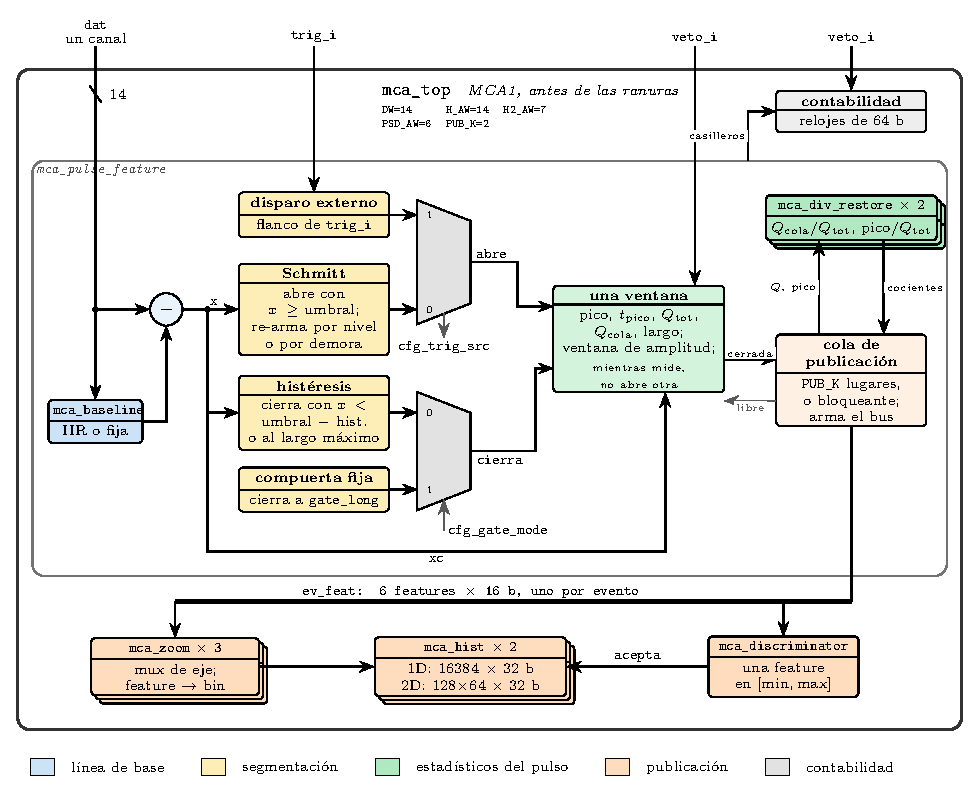
\includegraphics{apMCA_panorama_mca1}
\caption[Primera versión del MCA (MCA1)]{%
Primera versión del MCA (MCA1), antes de las ranuras y del banco de trapecios.
Una sola ventana mide un pulso a la vez: la abre el Schmitt propio sobre $x$ o
el flanco de \codigo{trig\_i}, y la cierra la histéresis o una compuerta fija.
Al cerrar, el resultado espera en una cola de \codigo{PUB\_K} lugares a que los
divisores calculen las \emph{features} de forma. No se dibujan la entrada ni el banco
de registros.\label{f:ap-mca-mca1}}
\end{figure}

\section{Elección de la cantidad de canales}
\label{S:ap-mca-canales}

Parecería natural determinar la cantidad de canales dada la resolución mínima
del sistema, o sea, poner un bin por cada una de las palabras de cuantización
que da el ADC. Esto claramente mantiene bajo el error de cuantización, pero este
no es el término de error dominante en nuestro sistema.

La \textbf{resolución máxima} del sistema está dada por la cuantización del
código de representación digital; según el modelo de la placa tenemos
diferentes precisiones. Para la \textbf{Z10 tenemos 14 bits}, mientras que las
placas especializadas en SDR (\emph{software defined radio}) presentan 16 bits.
Sin embargo, la cantidad de canales tiene sentido una vez que analizamos la
resolución efectiva, que \textbf{se fija por la SNR de la señal digitalizada}:
esta determina el poder resolutivo de las mediciones. Generalmente conviene ver
la \textbf{resolución efectiva} del sistema y elegir una resolución que asegure
que por \textbf{pico FWHM se tengan al menos 4} bines; esto se explica con la
corrección de Sheppard en la Sec.~\ref{S:implmca-fisher-bineado}.

Esto tiene sentido si hacemos el cálculo del presupuesto, que presenta el
siguiente cálculo:
\begin{equation}
  \text{Memoria necesaria [bytes]} = \underbrace{W_{bin}\,
  \text{[bytes]}}_{8} \times \underbrace{\text{Cantidad de bines}}_{> 4\,
  \text{FWHM/Res}}
  \label{e:ap-mca-memoria}
\end{equation}
Mientras que la memoria máxima está fija por el \textbf{recurso de memoria
empleado por el sistema}; en la Sec.~\ref{S:ap-mca-presupuesto} analizamos los recursos
presentes.

\subsection{Presupuesto de memoria por canal}
\label{S:ap-mca-presupuesto}

Los recursos lógicos de memoria en el PL son ambos \textbf{volátiles}. En la
Tabla~\ref{t:ap-mca-recursos} se presenta, en orden creciente, la cantidad total
de LUT6 y de RAMB36.

\begin{figure}[H]
\centering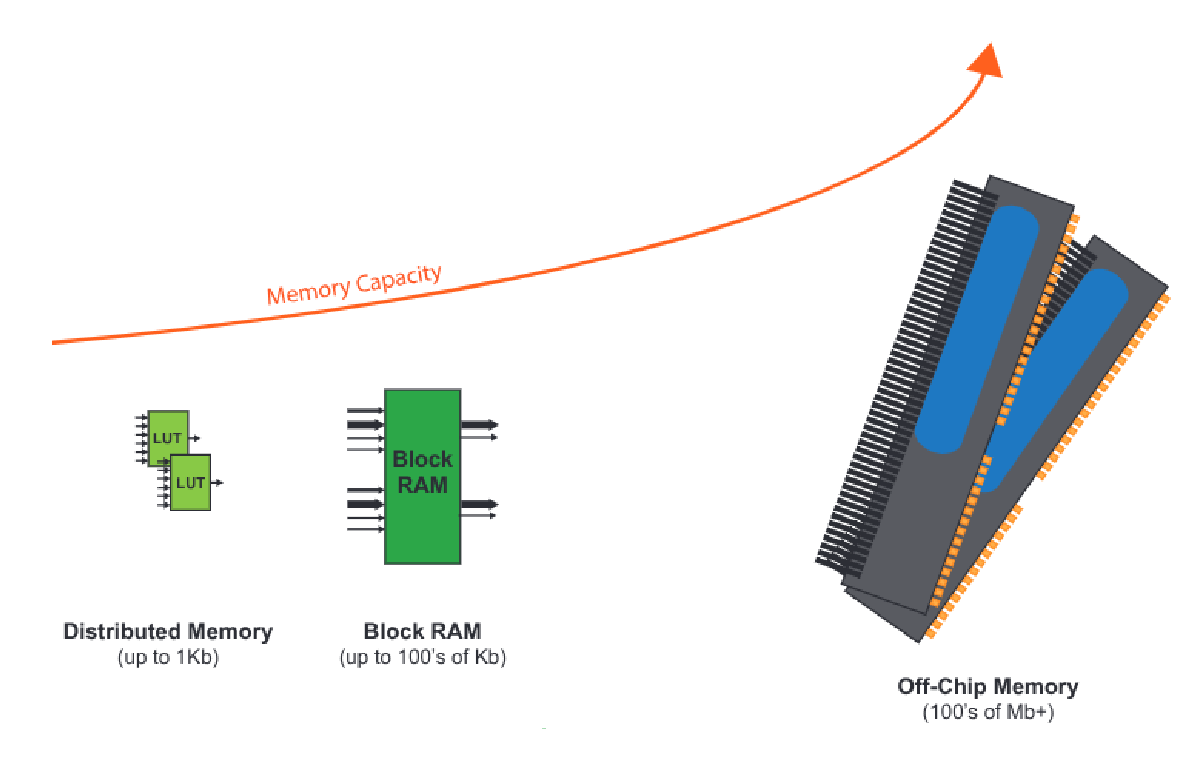
\includegraphics{apMCA_memoria_pl}
\caption[Recursos de memoria presentes en la plataforma]{%
Recursos de memoria presentes en la plataforma. De izquierda a derecha crece la
capacidad de cada tipo: la memoria distribuida en las LUT (hasta 1~kb por
bloque), la Block RAM (cientos de kb), la UltraRAM y la memoria externa. En la
Zynq-7000 de la Red Pitaya la PL tiene sólo las dos primeras; la UltraRAM es de
la familia UltraScale, y la memoria externa es la DDR, del lado del
PS.\label{f:ap-mca-memoria}}
\end{figure}

El aumento del tamaño se debe a la especialización de la arquitectura, en
particular a tener en cuenta menos puertos, es decir, cuántos valores de la
memoria se pueden leer o escribir de manera simultánea, y a su disposición,
distribuida o como HIP.

% En la nota la tabla tiene una columna "Tamano total" vacía; no se transcribe.
\begin{table}[H]
\centering
\caption[Recursos lógicos de la PL en los Zynq de Red Pitaya]{%
Recursos lógicos de la PL en los dos Zynq de la familia Red Pitaya: el XC7Z010,
de la placa que usamos, y el XC7Z020, de las variantes más grandes. La columna
$\times$ es la razón entre los dos.\label{t:ap-mca-recursos}}
\begin{tabular}{|l|r|r|r|}
\hline \encabezado \textbf{Recurso de la PL} & \textbf{XC7Z010} &
  \textbf{XC7Z020} & $\boldsymbol{\times}$ \\ \hline
LUT6 & 17\,600 & 53\,200 & 3.0 \\ \hline
Flip-flops & 35\,200 & 106\,400 & 3.0 \\ \hline
Block RAM (RAMB36) & 60 (2.1~Mb) & 140 (4.9~Mb) & 2.3 \\ \hline
\end{tabular}
\end{table}

Como consideración fundamental del diseño tomamos \textbf{anchos de contadores
de 32 bits}. Esto significa que con una \textbf{tasa de medición de 100~kcps}
concentrados en un pico, \textbf{saturar un bin lleva $\sim$12 horas}. Esta
decisión se justifica porque la alineación en potencias de dos es extremadamente
importante en una implementación barata; las alternativas son anchos de 16 o 64
bits.

El salto mayor en órdenes de magnitud en resolución y en el tamaño de los
contadores se obtiene a partir de \textbf{utilizar memoria \emph{off-chip}}; esto es
especialmente bueno para aumentar la resolución del histograma. El costo está en
la complejidad del \emph{buffering} y de la transferencia mediante el protocolo AXI a
la RAM, pero estas metodologías permiten \emph{throughputs} suficientes para tasas
altas.

\section{Poder resolutivo de Fisher en la elección del bineado}
\label{S:implmca-fisher-bineado}

Aumentar la cantidad de bines nos permite discriminar con mejor precisión; este
aumento de la precisión está acotado por el código digital empleado, si
consideramos
\begin{equation}
  \sigma_{ef}^2 = \sigma^2 + \Delta^2/12
  \label{e:ap-mca-sheppard}
\end{equation}
donde $\Delta$ es el ancho de cuantización. Con $\Delta = 1$ canal, la inflación
de $\sigma$ depende sólo de cuántos canales entran en un FWHM
(Tabla~\ref{t:ap-mca-inflacion}).

\begin{table}[H]
\centering
\caption[Inflación de $\sigma$ según los canales por FWHM]{%
Inflación de $\sigma$ por la cuantización según la cantidad de canales por
FWHM.\label{t:ap-mca-inflacion}}
\begin{tabular}{|l|c|c|c|c|c|}
\hline \encabezado \textbf{Canales / FWHM} & 1 & 2 & 4 & 8 & 16 \\ \hline
$\sigma$ inflado & \qty{20.9}{\percent} & \qty{5.6}{\percent} &
  \textbf{\qty{1.4}{\percent}} & \qty{0.36}{\percent} & \qty{0.09}{\percent}
  \\ \hline
\end{tabular}
\end{table}

De forma que se suelen pedir al menos 4 canales por FWHM, para no aumentar
$\sigma_{ef}$ en mucho más de un \qty{1}{\percent}.

\section{Mapa de registros}
\label{S:ap-mca-mapa}

En la Tabla~\ref{t:ap-mca-regmap} se presenta el mapa de registros de
\codigo{mca\_top}, con los desplazamientos respecto de la base del módulo. Todos
los registros son de 32 bits y podemos identificar siete secciones:
\begin{enumerate}
  \item \textbf{Identificación, control y estado}
    (\codigo{0x000}--\codigo{0x010}, \codigo{0x0A8}).
  \item \textbf{Configuración de la medición} (\codigo{0x01C}--\codigo{0x04C},
    \codigo{0x120}--\codigo{0x134}, \codigo{0x180}--\codigo{0x1A8}): la línea
    de base, la ventana de amplitud, las compuertas, las ranuras y el banco de
    trapecios.
  \item \textbf{Ejes, discriminador e histogramas}
    (\codigo{0x090}--\codigo{0x0A4}, \codigo{0x0B8}, \codigo{0x0BC}).
  \item \textbf{Contadores de eventos} (\codigo{0x050}--\codigo{0x064},
    \codigo{0x0AC}, \codigo{0x0B0}).
  \item \textbf{Relojes} (\codigo{0x068}--\codigo{0x07C},
    \codigo{0x0C0}--\codigo{0x0DC}, \codigo{0x0FC}, \codigo{0x100},
    \codigo{0x140}--\codigo{0x15C}), de 64 bits: leer la palabra baja congela la
    alta en un registro sombra, para que la lectura no se parta.
  \item \textbf{Períodos muertos, arribos y ranuras} (\codigo{0x0B4},
    \codigo{0x0E0}--\codigo{0x0F8}, \codigo{0x10C}--\codigo{0x11C}) y el
    \textbf{último evento} (\codigo{0x080}--\codigo{0x08C}).
  \item \textbf{Aperturas de los histogramas} (\codigo{0x10000} y
    \codigo{0x20000}).
\end{enumerate}

% Ocupa más de una página: longtable, para que se corte entre filas.
{\small
\begin{longtable}{|>{\raggedright\arraybackslash}p{0.15\textwidth}|c%
  |>{\raggedright\arraybackslash}p{0.2\textwidth}%
  |>{\raggedright\arraybackslash}p{\dimexpr0.65\textwidth-8\tabcolsep-5\arrayrulewidth-2.2em\relax}|}
\caption[Regmap del módulo \codigo{mca\_top}]{%
Regmap del módulo \codigo{mca\_top}, con \codigo{N\_ACC = 3} y tres formas en
el banco. Los \emph{offsets} que dejaron libres el Schmitt, la histéresis y la
publicación del MCA1 (\codigo{0x014}, \codigo{0x018}, \codigo{0x028},
\codigo{0x02C}, \codigo{0x048}, \codigo{0x104}, \codigo{0x108}), y los que
contaban pérdidas del re-armado (\codigo{0x0F0}, \codigo{0x114}), están
reservados: se escriben sin efecto y se leen en cero.\label{t:ap-mca-regmap}}
\\
\hline \encabezado \textbf{\emph{Offset}} & \textbf{Acc.} & \textbf{Nombre} &
  \textbf{Bits / descripción} \\ \hline
\endfirsthead
\hline \encabezado \textbf{\emph{Offset}} & \textbf{Acc.} & \textbf{Nombre} &
  \textbf{Bits / descripción} \\ \hline
\endhead
\codigo{0x000} & R & \codigo{MAGIC} & \codigo{0x4D434132} =
  \codigo{\textquotedbl MCA2\textquotedbl}, el mapa de las ranuras \\ \hline
\codigo{0x004} & R & \codigo{CAPS} & \codigo{[0]} espectro 1D; \codigo{[1]} mapa
  2D; \codigo{[2]} banco de trapecios \\ \hline
\codigo{0x008} & R & \codigo{WIDTHS} & \codigo{\{PSD\_AW[23:16], H2\_AW[15:8],
  H\_AW[7:0]\}} \\ \hline
\codigo{0x00C} & RW & \codigo{CTRL} & \codigo{[0]} \emph{run}; \codigo{[1]} \emph{clear}
  (pulso, autolimpiante): borra histogramas, contadores y relojes;
  \codigo{[8]} canal (0 IN1, 1 IN2) \\ \hline
\codigo{0x010} & R & \codigo{STATUS} & \codigo{[0]} \codigo{clear\_busy};
  \codigo{[1]} \codigo{busy} (alguna ranura ocupada); \codigo{[2]} base
  congelada demasiado tiempo; \codigo{[3]} veto; \codigo{[4]} disparo sin
  re-armar; \codigo{[5]} alguna ranura libre; \codigo{[9:8]} ranuras ocupadas
  \\ \hline
\codigo{0x0A8} & R & \codigo{FULL} & \codigo{[0]} \codigo{full\_1d};
  \codigo{[1]} \codigo{full\_2d}. Pegajosos: sólo los limpia \codigo{clear}
  \\ \hline
\codigo{0x01C} & RW & \codigo{cfg\_baseline} & \codigo{[13:0]} línea de base
  fija, con signo \\ \hline
\codigo{0x020} & RW & \codigo{cfg\_bl\_ctrl} & \codigo{[0]} seguidor IIR;
  \codigo{[7:4]} $k$, constante de tiempo $2^k$; \codigo{[31:16]} \emph{holdoff}, en
  muestras \\ \hline
\codigo{0x024} & R & \codigo{baseline\_now} & la línea de base que se está
  restando \\ \hline
\codigo{0x030}, \codigo{0x034} & RW & \codigo{cfg\_amp\_min/max} &
  \codigo{[15:0]} ventana de amplitud \\ \hline
\codigo{0x038} & RW & \codigo{cfg\_amp\_src} & \codigo{[0]} amplitud de la
  ventana (0 pico, 1 integral); \codigo{[12:8]} \codigo{q\_shift} de
  \codigo{F\_INT}. Escribirlo también elige \codigo{F\_PEAK} o \codigo{F\_INT}
  para el eje 1D y el x del 2D \\ \hline
\codigo{0x03C}, \codigo{0x040} & RW & --- & sin efecto; se conservan por
  compatibilidad \\ \hline
\codigo{0x044} & RW & \codigo{cfg\_dec} & \codigo{[15:0]} decimación propia del
  MCA (1 = sin decimar) \\ \hline
\codigo{0x04C} & RW & \codigo{cfg\_gate\_len} & \codigo{[15:0]} compuerta
  corta; \codigo{[31:16]} compuerta larga, en muestras desde el disparo
  \\ \hline
\codigo{0x120} & RW & \codigo{cfg\_n\_acc} & \codigo{[2:0]} ranuras habilitadas
  (0 se toma como 1) \\ \hline
\codigo{0x124} & RW & \codigo{cfg\_pre\_dly} & \codigo{[6:0]} retardo de la
  muestra respecto del disparo, en ciclos \\ \hline
\codigo{0x128} & RW & \codigo{cfg\_trap\_km} & forma 0: \codigo{[9:0]} $k$;
  \codigo{[25:16]} $m$. Escribirlo reinicia el estado del banco \\ \hline
\codigo{0x12C} & RW & \codigo{cfg\_trap\_mq} & \codigo{[19:0]} constante
  polo-cero, $16\,M$, común a todas las formas. Escribirlo reinicia el estado
  del banco \\ \hline
\codigo{0x130} & RW & \codigo{cfg\_trap\_med} & forma 0: \codigo{[15:0]}
  \codigo{off}; \codigo{[18:16]} \codigo{lw}; \codigo{[29:24]} escala
  \codigo{sh}; \codigo{[31]} (R) la región de la meseta entra en la compuerta
  \\ \hline
\codigo{0x134} & RW & \codigo{cfg\_n\_formas} & \codigo{[2:0]} formas que se
  usan; \codigo{[10:8]} (R) formas sintetizadas; \codigo{[31]} (R) los umbrales
  después de las formas en uso no superan la compuerta larga \\ \hline
\codigo{0x180}+16$\cdot$f & RW & \codigo{FORMA\_KM} f & como \codigo{0x128},
  para la forma f; la forma 0 es \codigo{0x128} \\ \hline
\codigo{0x184}+16$\cdot$f & RW & \codigo{FORMA\_MED} f & como \codigo{0x130},
  para la forma f; la forma 0 es \codigo{0x130} \\ \hline
\codigo{0x188}+16$\cdot$f & RW & \codigo{FORMA\_UMBR} f & \codigo{[15:0]}
  antes; \codigo{[31:16]} después: la forma f se elige si antes $\le$
  \codigo{F\_DTPREV} y después $\le$ \codigo{F\_DTNEXT} \\ \hline
\codigo{0x090} & RW & \codigo{cfg\_hist\_sel} & \emph{feature} de cada eje:
  \codigo{[3:0]} 1D; \codigo{[7:4]} x del 2D; \codigo{[11:8]} y del 2D
  \\ \hline
\codigo{0x094} & RW & \codigo{cfg\_zoom\_1d} & \codigo{[3:0]} $z$;
  \codigo{[15:8]} $k$; $z = 0$ es el rango completo \\ \hline
\codigo{0x0B8}, \codigo{0x0BC} & RW & \codigo{cfg\_zoom\_2dx/2dy} & ídem, para
  los dos ejes del 2D \\ \hline
\codigo{0x098} & RW & \codigo{cfg\_discr\_ctrl} & \codigo{[0]} habilita;
  \codigo{[1]} acepta afuera del intervalo; \codigo{[7:4]} \emph{feature} \\ \hline
\codigo{0x09C}, \codigo{0x0A0} & RW & \codigo{cfg\_discr\_min/max} &
  \codigo{[15:0]} intervalo del discriminador \\ \hline
\codigo{0x0A4} & RW & \codigo{cfg\_hist\_ctrl} & \codigo{[0]}
  \codigo{keep\_full}: seguir contando con un bin lleno \\ \hline
\codigo{0x050} & R & \codigo{cnt\_total} & ventanas cerradas \\ \hline
\codigo{0x054} & R & \codigo{cnt\_accepted} & eventos publicados \\ \hline
\codigo{0x058} & R & \codigo{cnt\_rej\_amp} & rechazados por la ventana de
  amplitud \\ \hline
\codigo{0x05C} & R & \codigo{cnt\_rej\_psd} & forma inválida: entran al 1D, no
  al 2D \\ \hline
\codigo{0x060} & R & \codigo{cnt\_pileup} & ventanas cerradas con marca de
  solape \\ \hline
\codigo{0x064} & R & \codigo{cnt\_dropped} & \codigo{cnt\_lost\_busy} más los
  \codigo{dropped} de los dos histogramas \\ \hline
\codigo{0x0AC} & R & \codigo{cnt\_rej\_discr} & rechazados por el
  discriminador \\ \hline
\codigo{0x0B0} & R & \codigo{cnt\_full\_supp} & incrementos suprimidos con un
  histograma lleno, de los dos \\ \hline
\codigo{0x068}, \codigo{0x06C} & R & \codigo{realtime} & palabras baja y alta
  \\ \hline
\codigo{0x070}, \codigo{0x074} & R & \codigo{livetime} & ídem \\ \hline
\codigo{0x078}, \codigo{0x07C} & R & \codigo{deadtime} & ídem \\ \hline
\codigo{0x0C0}, \codigo{0x0C4} & R & \codigo{vetotime} & ídem \\ \hline
\codigo{0x0C8}, \codigo{0x0CC} & R & \codigo{t\_win} & ídem \\ \hline
\codigo{0x0D0}, \codigo{0x0D4} & R & \codigo{t\_div} & ídem \\ \hline
\codigo{0x0D8}, \codigo{0x0DC} & R & \codigo{t\_rearm} & ídem \\ \hline
\codigo{0x0FC}, \codigo{0x100} & R & \codigo{t\_clear} & ídem \\ \hline
\codigo{0x140}+8$\cdot$j & R & \codigo{t\_ocup[j]} & ídem, con j = 0 \ldots{}
  \codigo{N\_ACC} \\ \hline
\codigo{0x0E0} & R & \codigo{cnt\_dead\_periods} & períodos muertos \\ \hline
\codigo{0x0E4} & R & \codigo{max\_dead\_len} & el período muerto más largo, en
  ciclos \\ \hline
\codigo{0x0E8} & R & \codigo{cnt\_dead\_ext} & períodos muertos con un disparo
  adentro \\ \hline
\codigo{0x0EC} & R & \codigo{cnt\_cross} & disparos con la adquisición en
  marcha \\ \hline
\codigo{0x0B4} & R & \codigo{cnt\_open} & disparos que abrieron una ranura
  \\ \hline
\codigo{0x0F4} & R & \codigo{cnt\_lost\_active} & perdidos sin ranura libre,
  con todas midiendo \\ \hline
\codigo{0x0F8} & R & \codigo{cnt\_lost\_veto} & perdidos por el veto \\ \hline
\codigo{0x110} & R & \codigo{cnt\_win} & ventanas abiertas; igual a
  \codigo{cnt\_open} \\ \hline
\codigo{0x118} & R & \codigo{cnt\_trig} & flancos de \codigo{trig\_i}, haya
  adquisición o no \\ \hline
\codigo{0x10C} & R & \codigo{PUB\_OCC} & \codigo{[7:0]} ranuras cerradas
  esperando al publicador; \codigo{[15:8]} su máximo; \codigo{[31:16]} número
  de la última ventana publicada \\ \hline
\codigo{0x11C} & R & \codigo{N\_ACC} & ranuras sintetizadas \\ \hline
\codigo{0x080}--\codigo{0x08C} & R & último evento & amplitud, forma, $Q_{tot}$
  y $Q_{cola}$ del último evento publicado, para depurar \\ \hline
\codigo{0x10000} & R & espectro 1D & $2^{13}$ palabras de 32 bits \\ \hline
\codigo{0x20000} & R & mapa 2D & $128 \times 64$ palabras de 32 bits \\ \hline
\end{longtable}}

% Bibliografía de este apéndice.
\bibliografiacapitulo

%%% Local Variables:
%%% mode: latex
%%% TeX-master: "template"
%%% End:
